% FUNDAMENTAÇÃO TEÓRICA--------------------------------------------------------

\chapter{FUNDAMENTAÇÃO TEÓRICA}
\label{chap:fundamentacao-teorica}

Neste capítulo, serão abordados os aspectos teóricos necessários para o melhor discernimento das definições e componentes a serem utilizados ao longo do projeto. De início, serão abordados os conceitos base como redes \textit{Wireless}, \textit{Internet of Things}, \textit{Smart Things} e o protocolo \textit{MQTT}. Conceitos como a montagem de circuitos eletrônicos, sensoriamento, implementação de sistemas embarcados assim como as tecnologias envolvidas na criação de aplicações \textit{mobile} e \textit{desktop} também serão tratadas neste capítulo. As subseções posteriores, agruparão os conceitos em elementos: de base, de \textit{Hardware},  de \textit{Firmware} e de \textit{Software}.  

\section{Elementos Base}

Esta seção discorre sobre as tecnologias e metodologias que serão utilizadas em todas as vertentes deste trabalho, destacando-se as partes mais relevantes.

\subsection{Redes \textit{Wireless}}

O termo \textit{Wireless} provém do inglês: \textit{wire} (fio, cabo); less (sem); caracteriza qualquer tipo de conexão para transmissão de sem a utilização fios ou cabos \cite{redeswireless}. É importante notar que uma rede sem fio possibilita um conjunto de equipamentos conectados através de sinais de rádio frequência possuindo vantagens cruciais para a aplicação do conceito de Internet das Coisas:

\begin{itemize}
	\item \textbf{Maior produtividade - } disponibiliza acesso à rede em todo o raio de alcance onde o ponto de acesso está instalado, oferecendo liberdade de deslocamento com conexão contínua;
	
	\item \textbf{Flexibilidade de instalação -} podem ser instaladas em locais com temperaturas elevadas, em que os cabos não suportariam, ou em locais que necessitam de acesso temporário;
	
	\item \textbf{Redução de custo - } reduzem os custos de instalação, dispensando o uso de material para cada ponto de conexão;
	
	\item \textbf{Interoperabilidade e segurança - } capaz de comunicar sistemas de forma confiável e com segurança, possuindo chaves de acesso e até mesmo transferindo mensagens criptografadas.   

\end{itemize}

Dentre as diversas características podemos destacar que as redes \textit{wireless} são dividas quanto a \textbf{abrangência de sinal} em:

\begin{itemize}
	\item \textbf{\textit{Wireless Local Area Network} - WLAN - } rede de área local;
	\item \textbf{\textit{Wireless Metropolitan Area Network} - WLAN - } rede de região metropolitana;
	\item \textbf{\textit{Wireless Wide Area Network} - WWAN - } rede de área mundial sem fio;
	\item \textbf{\textit{Wireless Local Loop} - WLL - } acesso fixo sem fio;
	\item \textbf{\textit{Wireless Personal Area Network} - WPAN} - redes pessoais sem fio;
\end{itemize}

Fundado em 1987, o grupo de trabalho \textit{Institute of Electrical and Electronics Engineers} - \textit{IEEE} 802.11\textit{ Wireless LAN}, realizou a padronização das \textit{WLANs}. Desenvolveu-se o padrão DS-SS IEEE 802.11b, chamado de \textit{Wi-Fi} pela \textit{Wireless Ethernet Compatibility Alliance} - WECA o qual é amplamente usado no mercado atual. \cite{internetdascoisassemmisterios}. A partir dessa padronização é possível aplicar as transmissões de dados por diversos protocolos de maneira barata e prática.

A topologia de uma rede IEEE 802.11 (\textit{Wi-Fi})  possui os seguintes elementos-chave:

\begin{itemize}
	\item \textbf{BSS - \textit{Basic Service Set} -} corresponde a uma célula de comunicação \textit{wireless};
	\item \textbf{STA - \textit{Stations} -} são as estações de trabalho que comunicam-se entre si dendo da \textbf{BSS};
	\item \textbf{AP - \textit{Access Point} -} coordena a comunicação entre as \textbf{STA's} dentro da \textbf{BSS}. Na maioria das vezes roteadores realizam tal operação;
	\item \textbf{\textit{Bridge} -} faz a ligação entre diferentes redes, por exemplo, uma rede sem fio para uma rede cabeada convencional;
	\item  \textbf{ESS - \textit{Estended Service Set} -} consiste de várias células \textbf{BSS's} vizinhas que se interceptam e cujos \textbf{AP's} estão conectados a uma mesma rede tradicional. Nestas condições uma \textbf{STA} pode movimentar-se de um \textbf{BSS} para outr, permanecendo conectada à rede. Este processo é denominado \textit{Roaming}.
\end{itemize}

\subsection{A Internet das Coisas}

Existe uma diversidade de ideias em relação ao conceito de Internet das Coisas (\textit{Internet of Things - IoT}), sendo que todos os conceitos, em resumo, fazem alusão à um conjunto de tecnologias e protocolos associados que permitem que objetos se conectem a uma rede de comunicações e onde são identificados e controlados.

Esse termo se tornou possível graças aos avanços tecnológicos e as reduções de custo de todos os dispositivos eletroeletrônicos, os quais possuem a capacidade de comunicação principalmente por meio de protocolos \textit{Wiress} (\autoref{fig:iot_protocols}). Com a aplicação em massa do \textit{IoT} surge a \textit{hiperconectividade}, termo que descreve a possibilidade da aquisição descomunal de informações as quais podem ser utilizadas para melhorar um processo, produto ou serviço.

\begin{figure}[H]
	\centering
	\caption{Protocolos utilizados para aplicacão do \textit{IoT} com base nos conceitos de redes. Relação entre velocidade-força e distância.}
	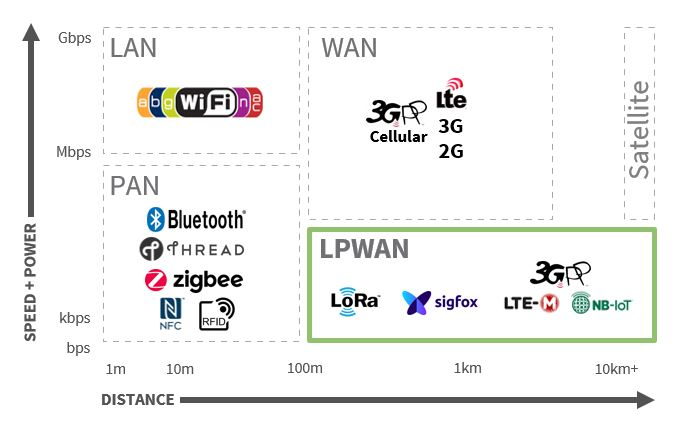
\includegraphics[width=0.8\textwidth]{figuras/iotprotocols.jpg}
	\fonte{iot.do, 2021}
	\label{fig:iot_protocols}
\end{figure}


\subsection{O protocolo MQTT}

O protocolo \textbf{\textit{Message Queuing Telemetry Transport}} - MQTT foi inventado e desenvolvido inicialmente pela \textit{International Business Machines} - IBM no final dos anos 90. Sua aplicação original era vincular sensores em \textit{pipelines} de petróleo a satélites. 

Como seu nome sugere, ele é um protocolo de mensagem com suporte para a comunicação \textbf{assíncrona} entre as partes. Um protocolo de sistema de mensagens assíncrono desacopla o emissor e o receptor da mensagem tanto no espaço quanto no tempo e, portanto, é escalável em ambientes de rede que não são confiáveis. Apesar de seu nome, ele não tem nada a ver com filas de mensagens, na verdade, ele usa um modelo de publicação e assinatura. No final de 2014, ele se tornou oficialmente um padrão aberto OASIS, com suporte nas linguagens de programação populares, usando diversas implementações de \textit{software} livre \cite{IBM}.

O MQTT foi projetado para aplicações que utilizam pouca banda de rede, com requisitos de \textit{hardware} extremamente simples e leve. Ele está na mesma camada OSI que o \textbf{\textit{Hypertext Transfer Protocol}} - HTTP, porém a maior diferença entre eles é o tamanho do \textit{payload}. No HTTP o \textit{payload} \footnote{\textit{\textbf{payload}} - Dado de interesse sem metadados, sem cabeçalho de transmissão ou outras informações acessórias usadas apenas como infraestrutura para transmitir o que importa.} é maior, o que inviabiliza o uso em conexões de baixa qualidade. Além disso o MQTT possui maior segurança, apresenta mais níveis de serviço, é menos complexo e permite uma comunicação de 1 para N se comparado ao HTTP que também é um protocolo utilizado no universo de Internet das Coisas \cite{UFRJ}.

Em uma rede MQTT existem dois agentes principais: o \textit{\textbf{broker}} e os \textit{\textbf{clients}}. O \textit{broker} é um servidor que centraliza as mensagens dos clientes e as encaminha para os clientes interessados. Já o cliente é um dispositivo ou serviço que tenha capacidade de interagir com o \textit{broker} e trocar mensagens. Podemos exemplificar como tipos de clientes (\autoref{fig:mqtt_diagram}) um sensor, um controlador, um atuador ou até mesmo um \textit{software} sendo executado em alguma instância da rede.

\begin{figure}[H]
	\centering
	\caption{Diagrama básico MQTT}
	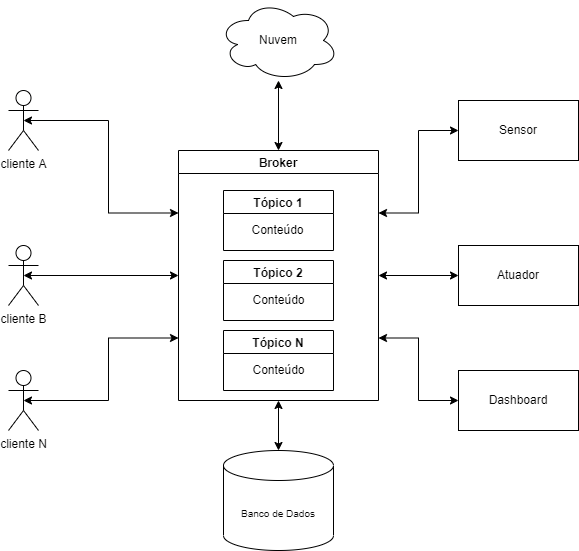
\includegraphics[width=0.8\textwidth]{figuras/mqtt.drawio.png}
	\fonte{própria, 2021}
	\label{fig:mqtt_diagram}
\end{figure}

Como qualquer outro protocolo de comunicação o MQTT possui diversos termos e características associadas, como a segurança, a definição dos \textit{endpoints}\footnote{\textbf{endpoints} - Pontos de extremidade. Terminais de conexão entre uma API e o cliente.}, o endereçamento, tipo de dado trafegado, entre outros. Abaixo estão pontuados os dados cruciais para a aplicação deste trabalho.

\begin{itemize}
	\item \textbf{\textit{broker}}: é o intermediário no processo de comunicação, atuando como um servidor;
	\item \textbf{\textit{client}}: responsável por estabelecer e manter uma conexão com o \textit{broker}, enviar e receber as mensagens;
	\item \textit{\textbf{broker ip}}: identificação única do servidor \textit{\textbf{broker}} conectado em determinada rede;
	\item \textbf{\textit{broker username e broker password}}: credenciais, opcionais, para determinado cliente estabelecer conexão com o servidor; 
	\item  \textit{\textbf{QoS}}: nível de qualidade do serviço desejado, indicando como deve ser a relação entre os elementos comunicantes. \textit{QoS 0}: Não há a confirmação de entrega de uma mensagem e quem a envia não tem obrigação de manter a mensagem armazenada para futuras retransmissões. \textit{QoS 1}: Existe a confirmação de entrega da mensagem. As mensagens enviadas são armazenadas por quem as envia. \textit{QoS 2}: Garante que a mensagem seja entregue exatamente uma vez, com envio de confirmações de recebimento e confirmações de recebimento de confirmações de recebimento. Enquanto uma mensagem não é confirmada, ela é mantida.\cite{fabiobrandao}
	
	\item \textbf{\textit{last good message}}: é a operação à qual o \textit{broker} envia a última menagem válida recebida em um determinado tópico ao ser requisitado por um cliente. Normalmente, se um cliente MQTT assina um tópico em um \textit{broker}, ele não receberá nenhuma das mensagens publicadas nele antes da assinatura. Se um cliente publicar uma mensagem em um tópico com o sinalizador de retenção definido como \textit{True}, o corretor salvará essa mensagem como a “Última Mensagem válida” nesse tópico. Esta mensagem será recebida por qualquer cliente que assine esse tópico \cite{mntolia}. 
	
	\item \textbf{\textit{last will testament (LWT)}}: são mensagens pré-definidas a serem publicadas pelo broker em nome de um determinado cliente, uma vez que esse cliente está \textit{offline} e não pode publicar mais.
	\item \textbf{\textit{keep alive}}: mensagens periódicas enviadas por determinado cliente buscando validar a conexão;
	\item \textbf{tópicos, \textit{publish} e \textit{subscribe}}: O ato de um cliente enviar uma mensagem é chamado \textit{publish}(publicação). E para receber mensagens de determinado um tópico um cliente deve fazer um \textit{subscribe}(inscrição). Os níveis de um tópico são separados por “/” e um cliente pode optar por se inscrever em quantos tópicos forem necessários, utilizando os artifícios da \autoref{tab:simbolos_mqtt}.
	
\end{itemize}

\begin{table}[H]
	\centering
	\resizebox{\textwidth}{!}{%
		\begin{tabular}{c|c|c}
			\hline
			Símbolos & Descrição & Exemplo \\ \hline
			+ & Retorna ou envia qualquer informação naquele nível (Coringa) & \begin{tabular}[c]{@{}c@{}}area/10/sensor/5000/temperatura\\ area/10/sensor/4000/temperatura\\ area/10/sensor/+/temperatura\end{tabular} \\ \hline
			\# & Retorna ou envia qualquer coisa abaixo daquele nível & area/10/\# \\ \hline
			\$ & Tópicos iniciados com \$ são especiais usados internamente pelo broker. & \$SYS/broker/clients/total \\ \hline
		\end{tabular}%
	}
	\caption{Caracteres especiais utilizados para envio e recebimento no protocolo MQTT.}
	\label{tab:simbolos_mqtt}
\end{table}

\section{Elementos de \textit{Hardware}}
\subsection{O microcontrolador ESP8266}

O \textit{ESP8266} (\autoref{fig:esp8266ex}) é um \textit{chip} microcontrolador da fabricante chinesa \textit{Espressif Systems} construído em torno de um processador Tensilica Xtensa LX3, inclui \textit{Wi-Fi on-board}. Originalmente concebido como um adaptador \textit{UART} para \textit{Wi-Fi} (utilizado em \textit{tablets}), permitindo que outros microcontroladores se conectem a uma rede \textit{Wi-Fi} e façam conexões \textit{TCP/IP} simples usando comandos do estilo \textit{Hayes}\footnote{\textbf{comandos \textit{Hayes}:} série de \textit{strings} curtas que podem ser combinadas para produzir comandos de operações como discar, desligar e alterar os parâmetros de conexão.}, o \textit{ESP8266} rapidamente se tornou popular como um microcontrolador autônomo devido ao seu baixo custo de mercado.

\begin{figure}[H]
	\centering
	\caption{\textit{ESP8266EX}.}
	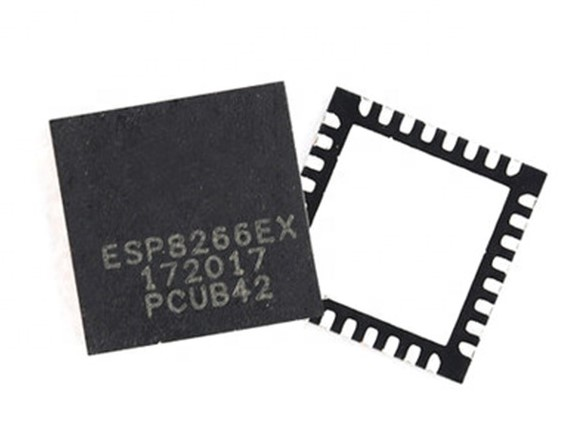
\includegraphics[width=0.3\textwidth]{figuras/esp8266ex.jpg}
	\fonte{DIGIKEY, 2020}
	\label{fig:esp8266ex}
\end{figure} 

Apesar da falta de documentação inicial, uma grande comunidade foi formada em
torno do ESP8266, integrando e dando suporte ao \textit{firmware} para o chip, fazendo-o compatível com a plataforma \textit{Arduino}.
Embora o chip \textit{ESP8266} seja feito pela \textit{Espressif}, existem diversos módulos criados para aplicações distintas.

Os modelos podem se diferenciar pela quantidade de pinos extenados, memória \textit{flash} instalada, modelo de antena, entre outros. Para a realização deste trabalho foram escolhidos os modelos: \textit{ESP-12S} (\autoref{fig:esp12s}) e \textit{ESP-12E} (\autoref{fig:esp12e}) presentes, respectivamentes nas placas de desenvolvimento WEMOS D1 e NodeMCU. Ambos possuem 11 \textit{GPIOs - General Purpose Input Output} sendo ideais para a leitura de uma gama de sensores. A diferença entre ambos está no desenho da antena integrada, sendo a do ESP-12S mais otimizada e, na quantidade de pinos externados, o ESP-12S não extena os pinos voltados para conexão \textit{SPI} e de cartões \textit{SD} \cite{esp8266}. As características gerais e específicas para o densenvolvimento deste trabalho estão descritas no \textbf{anexo A}. 


\begin{figure}[H]
	\centering
	\caption{Vista superior do \textit{ESP-12S}.}
	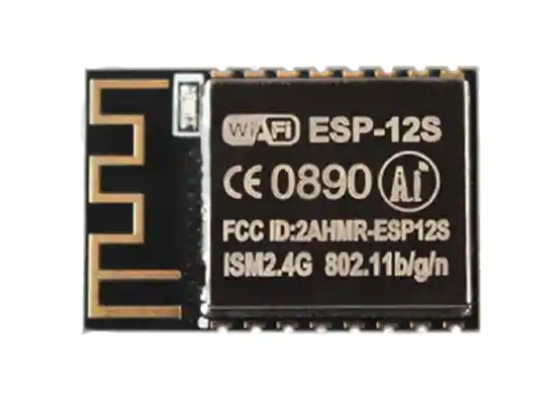
\includegraphics[width=0.3\textwidth]{figuras/ESP-12S.png}
	\fonte{FILIPEFLOP, 2020}
	\label{fig:esp12s}
\end{figure} 

\begin{figure}[H]
	\centering
	\caption{Vista superior do \textit{ESP-12E}.}
	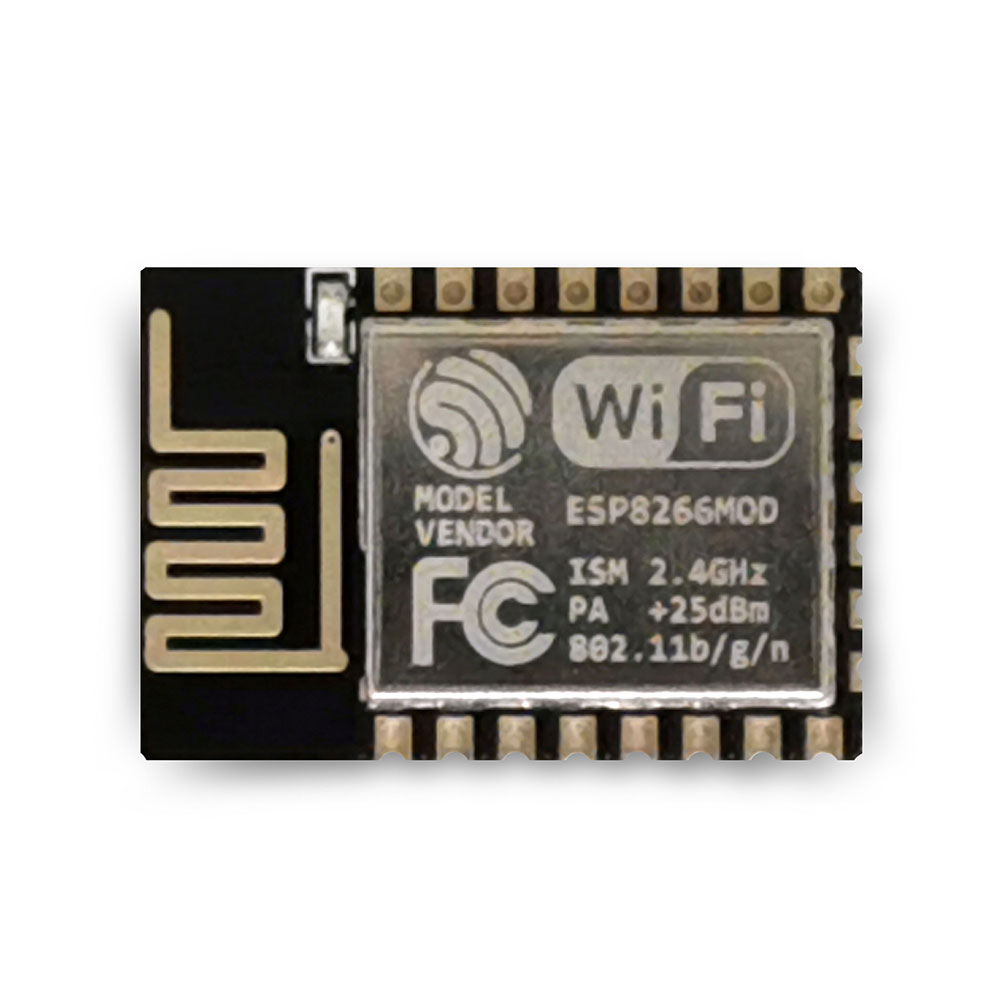
\includegraphics[width=0.3\textwidth]{figuras/ESP-12E.png}
	\fonte{FILIPEFLOP, 2020}
	\label{fig:esp12e}
\end{figure}

\begin{figure}[H]
	\centering
	\caption{Wemos D1 com ESP-12S.}
	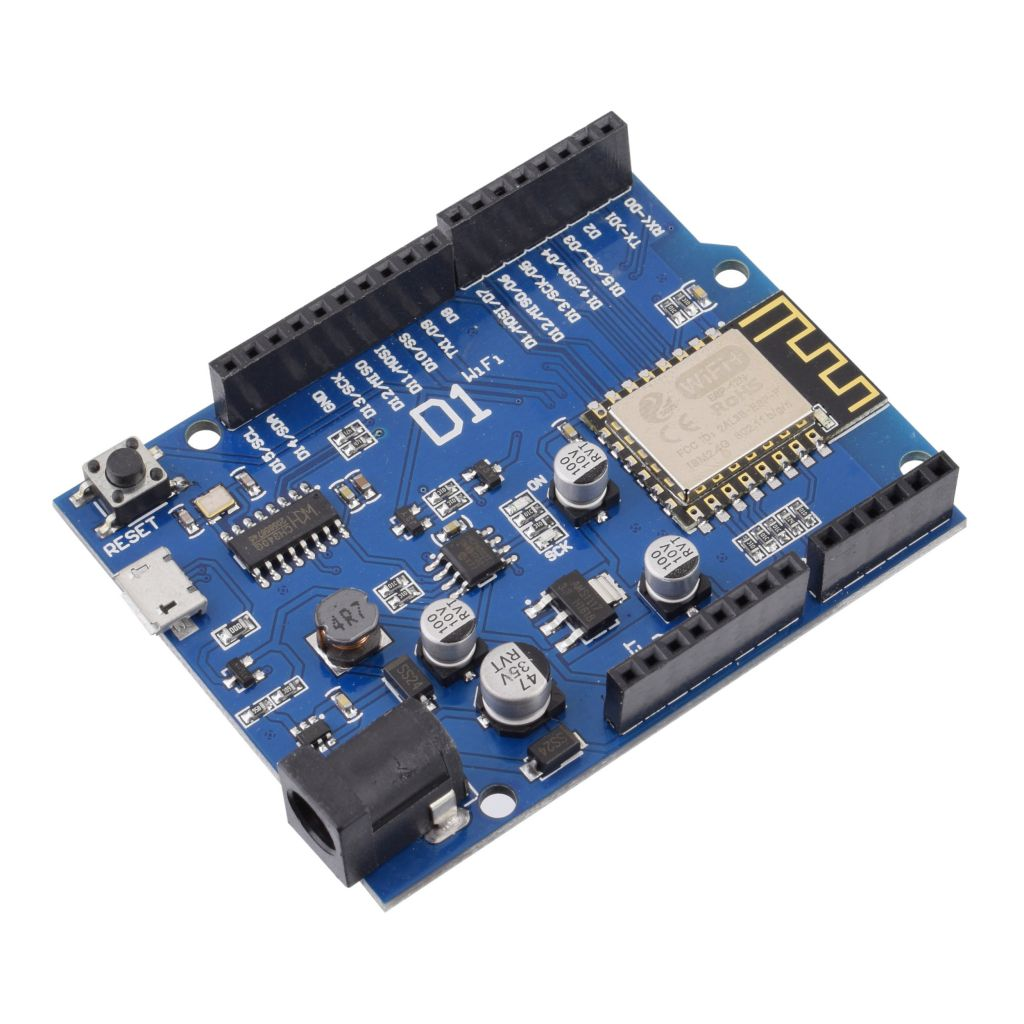
\includegraphics[width=0.3\textwidth]{figuras/ESP-12S-wemos.png}
	\fonte{esp8266.org, 2021}
	\label{fig:esp12s-wemos}
\end{figure}

\begin{figure}[H]
	\centering
	\caption{Nodemcu com ESP-12E.}
	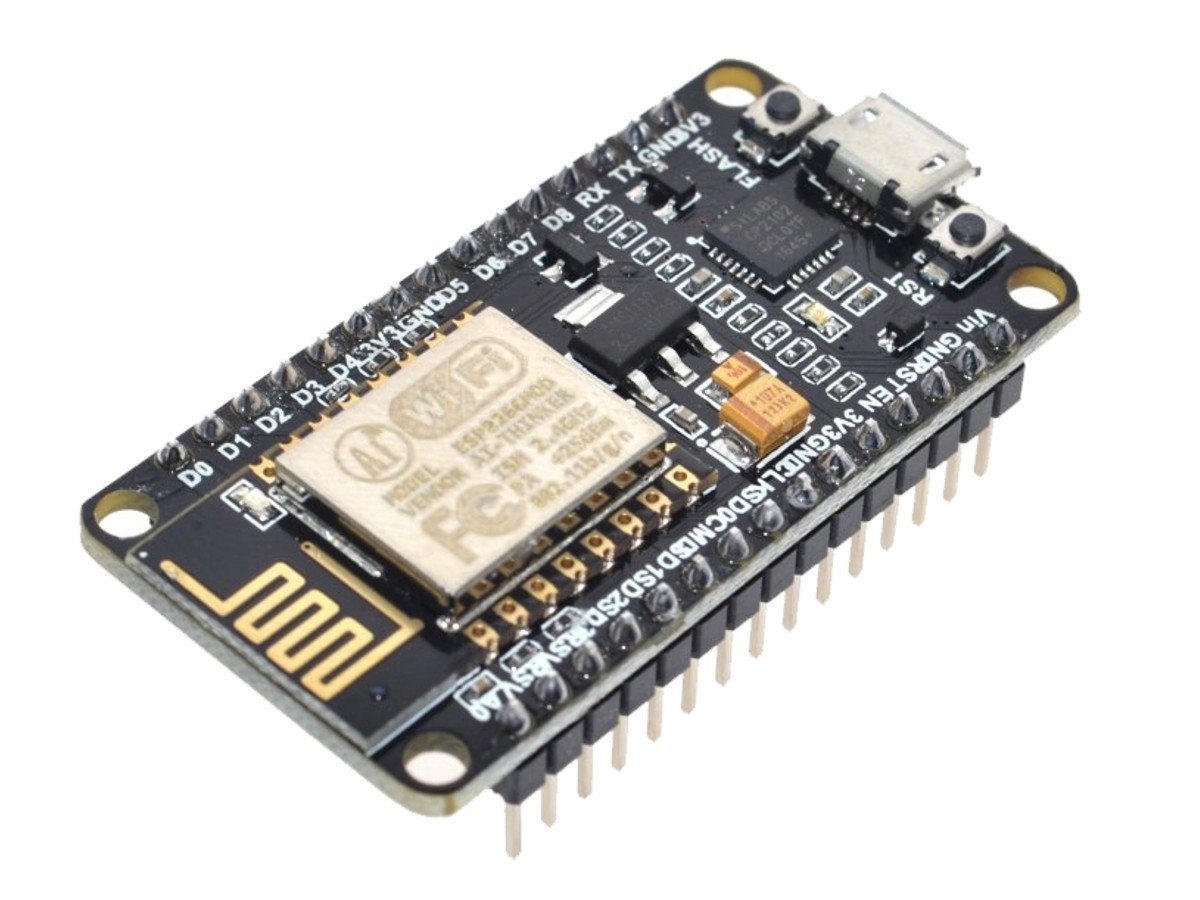
\includegraphics[width=0.3\textwidth]{figuras/ESP-12E-nodemcu.png}
	\fonte{esp8266.org, 2021}
	\label{fig:esp12s-nodemcu}
\end{figure}







\subsection{A Raspberry Pi Zero W}

A \textit{Raspberry Pi Zero W} é basicamente um computador de placa única. Ela possui recursos como \textit{slot} para cartão \textit{microSD}, conectores \textit{HDMI} e de câmera, conectividade \textit{Wi-Fi} e \textit{Bluetooth 4.0}, um conector macho de entrada-saída (\textit{GPIO}) de 40 pinos e mini conector de alimentação \textit{+ 5VDC}. O microcontrolador baseado no processador \textit{BCM2835 ARMv7 system-on-chip (SoC)} alimenta o Pi Zero W.

Essa versão de \textit{hardware} da \textit{Raspberry Pi Foundation} é muito compacta, ficando no meio termo entre as fazes de prototipação e aplicação. Com o microprocessador \textit{ARM BCM2835} de \textit{1GHz}, memória \textit{RAM} de \textit{512MB} e um sistema operacional enxuto instalado, a \textit{Raspberry Pi Zero W} é ideal para rodar aplicações como um \textit{Broker MQTT}. Informações adicionais sobre esse dispositivo estão disponíveis no \textbf{Anexo B}.

\begin{figure}[H]
	\centering
	\caption{Vista superior da \textit{Raspberry Pi Zero W}}
	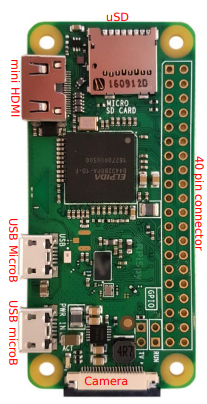
\includegraphics[width=0.3\textwidth, angle = 90]{figuras/rasp_zerow.png}
	\fonte{SPARKFUN, 2020}
	\label{fig:rasppizerow}
\end{figure} 

\subsection{As fontes de alimentação DC}

Para alimentação elétrica de todos os dispositivos eletrônicos envolvidos no processo de automação da cisterna, foram utilizadas dois tipos de fontes chaveadas: de \textit{12V/20A} para o módulo \textbf{CCM} e \textit{12V/10A} para o módulo \textbf{TCM}, representadas pela \autoref{fig:fontechaveada}. Essas fontes são ideais por possuir características robustas, como proteção eletromecânica e potência necessária para ativação de motores e válvulas solenoides. Há também a disponibilização de vários conectores na saída, os quais podem ser interligados para pontos específicos de alimentação.

\begin{figure}[H]
	\centering
	\caption{Vista superior da fonte}
	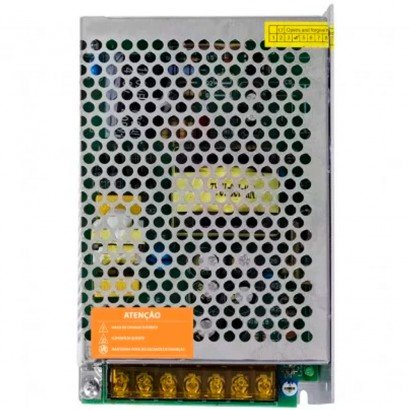
\includegraphics[width=0.4\textwidth]{figuras/fonte_chaveada.jpg}
	\fonte{AMAZON, 2020}
	\label{fig:fontechaveada}
\end{figure} 

\subsection{A motobomba ou bomba d'água}

A bomba d'água selecionada, \autoref{fig:bomba} , trabalha com fontes de alimentação de correntes contínuas (\textit{DC}) o que permite um maior controle do funcionamento através de sistemas \textit{microprocessados}. Essa bomba opera a \textit{12V}, com potência máxima de \textit{80W}. Ela possui a capacidade de exercer uma vazão de \textit{5,5L/min} com ganho de elevação de no máximo 40\textit{m}.

\begin{figure}[H]
	\centering
	\caption{Bomba d'água \textit{DC}}
	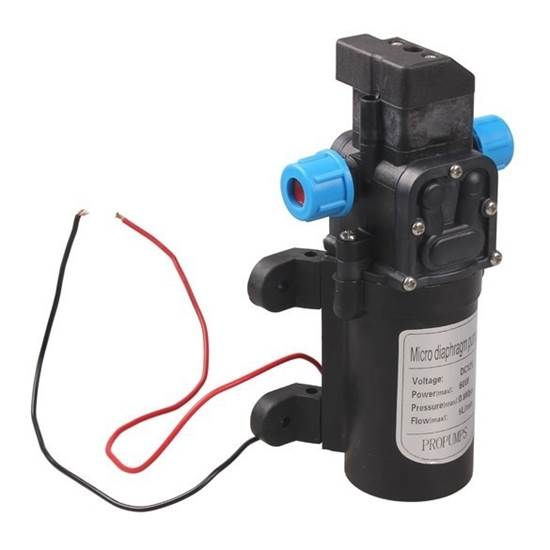
\includegraphics[width=0.3\textwidth]{figuras/bomba.jpeg}
	\fonte{ENERGIA TOTAL, 2020}
	\label{fig:bomba}
\end{figure}

\subsection{O sensor ultrassônico}
\label{ssec:sensor_ultra}

Um sensor ultrassônico é um instrumento que mede a distância até um objeto usando ondas sonoras de frequência acima do alcance da audição humana (ultrassônicas). Ele usa um transdutor para enviar e receber pulsos ultrassônicos os quais são utilizados para medição de distância através de lapsos temporais (\autoref{fig:operacao_ultrassonico}). A equação de distância associada é dada por:

\begin{equation}
d = \frac{\Delta t \cdot v}{2}
\end{equation}
\\
\begin{itemize}
	
	\item $d$ é a distância;
	\item $\Delta t$ é a diferença entre o tempo de emissão e chegada da onda;
	\item  $v$ é a velocidade do som (tomada como $340m/s$). \\
\end{itemize}





\begin{figure}[H]
	\centering
	\caption{Representação do funcionamento de um sensor ultrassônico}
	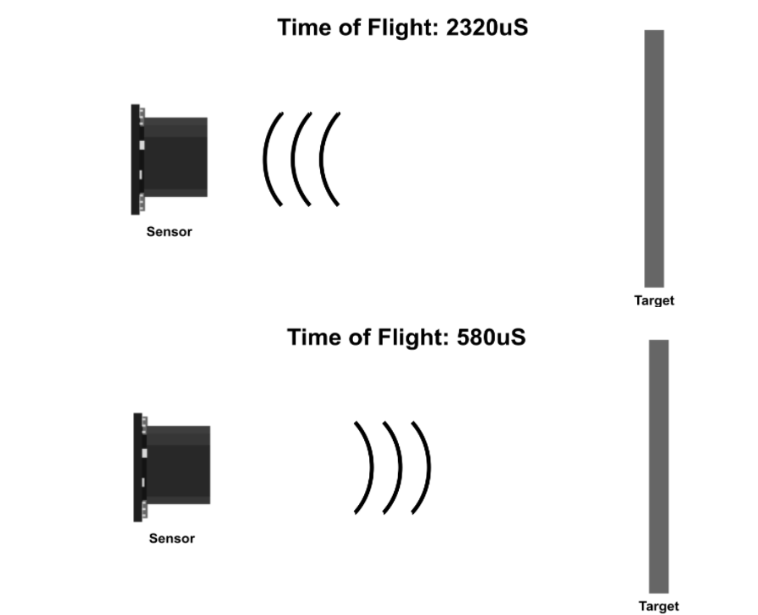
\includegraphics[width=0.6\textwidth]{figuras/ultrassonico_operacao.png}
	\fonte{Maxbotix, 2021}
	\label{fig:operacao_ultrassonico}
\end{figure}

Para medição de nível selecionou-se o módulo ultrassônico \textit{JSN-SR04T}. Esse módulo oferce uma região de medição de distância entre $20 cm$ a $600 cm$, com precisão na faixa de $2 mm$.

Esse módulo de apenas quatro pinos: \textit{5V} (VCC), \textit{Trig (RX)}, \textit{Echo (TX)} e \textit{GND}, inclui um transceptor integrado além do seu circuito de controle o qual possui três modos de operação sendo selecionados pelo valor do resistor (R27) soldado a placa:


\begin{itemize}
	\item \textbf{Modo de operação 1 (R27 não soldado)}: neste modo, o microcontrolador na placa não é utilizado. As operações de leitura ficam por responsabilidade externa. 
	
	\item \textbf{Modo de operação 2 (R27 $= 47k\Omega$)}: neste modo, o microcontrolador da placa entra em modo de leitura constante e envia dados a cada $100ms$. Os dados são enviados via o pino TX respeitando o protocolo: 0XFF + HIGH DATA + LOW DATA + SUM 1.
	
	\item \textbf{Modo de operação 3 (R27 $= 120k\Omega$)}: neste modo, o microcontrolador entra em modo de baixo consumo e só envia os dados de leituras ao ser acionado pelo pino RX. Se a mensagem de acionamento for 0X55, a leitura de distância é enviada pelo TX da mesma forma do modo anterior. \\
\end{itemize}

Sobre o protocolo utilizado, cada parte da mensagem tem a seguinte definição:

\begin{itemize}
	\item 0xFF: indica a chegada de uma mensagem;
	\item HIGH DATA: 8 bits mais significativos da leitura;
	\item LOW DATA: 8 bits menos significativos da leitura;
	\item SUM 1: O resultado da soma de todos os caracteres (0XFF + HIGH DATA + LOW DATA) para que a mensagem seja validada.
\end{itemize}



\begin{figure}[H]
	\centering
	\caption{Sensor ultrassônico JSN-SR04T.}
	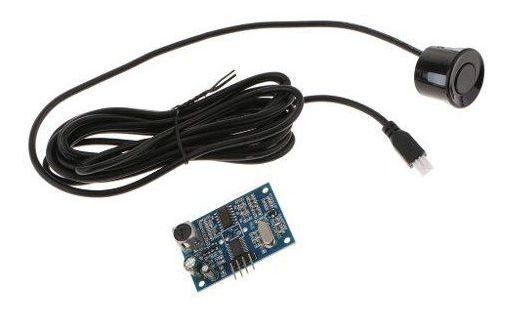
\includegraphics[width=0.5\textwidth]{figuras/sensor_ultra.jpg}
	\fonte{USINAINFO, 2020}
	\label{fig:sensor_ultra}
\end{figure}

O transceptor, resistente à água e poeira, é conectado ao módulo por meio de um cabo com \textit{2,5 metros} de comprimento. 


\subsection{A válvula solenoide}

Uma válvula solenoide (\autoref{fig:valvula_solenoide}) é um tipo de válvula que pode ser acionada ou desacionada eletronicamente. Seu componente principal é uma bobina elétrica com um núcleo ferromagnético móvel no centro chamado de êmbolo.

Dependendo da aplicação, uma válvula pode ser classifica em \textbf{Normalmente Aberta - NA} ou\textbf{ Normalmente Fechada - NF}. Para uma \textbf{NF}, em sua posição de repouso, o êmbolo tampa um pequeno orifício por onde é capaz de circular um fluído. Quando uma corrente elétrica circula na bobina, cria um campo magnético o qual exerce força sobre o êmbolo. Ele é deslocado em direção ao centro da bobina, abrindo o orifício e possibilitando a passagem do fluído. A operação para uma válvula \textbf{NA} é justamente o oposto, o êmbolo fica no centro e é deslocado com a formação do campo magnético. Outra classificação é quanto ao número de vias e as formas de controle. Para este trabalho nos atentaremos para válvulas de duas vias com retorno por mola, representadas na figura abaixo.

\begin{figure}[H]
	\centering
	\caption{Representação de válvulas: \textit{(a)} Normalmente Fechada  e \textit{(b)} Normalmente Aberta. Ambas de duas vias.}
	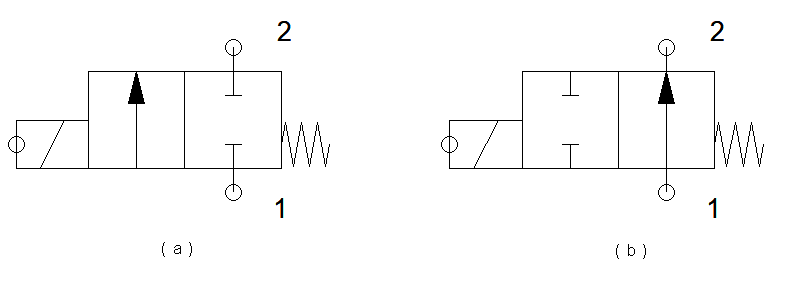
\includegraphics[width=0.7\textwidth]{figuras/valvulas.png}
	\fonte{Própria, 2021}
	\label{fig:valvulas}
\end{figure}

\begin{figure}[H]
	\centering
	\caption{Representação interna de uma válvula solenoide com seus principais componentes}
	\includegraphics[width=0.4\textwidth]{figuras/válvula_solenoide.png}
	\fonte{Citisystems, 2021}
	\label{fig:valvula_solenoide}
\end{figure}

Alguns exemplos do uso de válvulas solenoides incluem sistemas de aquecimento, tecnologia de ar comprimido, automação industrial, piscinas, sistemas de aspersão, máquinas de lavar roupa, equipamentos odontológicos, sistemas de lavagem de carros e sistemas de irrigação \cite{Citisystems}.

O modelo de válvula solenoide utilizada foi da marca Nascimetal (\autoref{fig:solenoide}) a qual possui características como:  \textit{1/2"} x \textit{1/2"}, tensão de operação em torno de \textit{12V} \textit{DC}, consumo médio, quando ativada, de \textit{500mA}, pressão de operação à $8,0 kgf/cm^2$ com vazão máxima de $40L/min$ e vida útil de 50 mil operações. Garantiu o controle do fluxo de água de acordo com os dados elétricos enviados pelo microcontrolador.

\begin{figure}[H]
	\centering
	\caption{Válvula solenoide}
	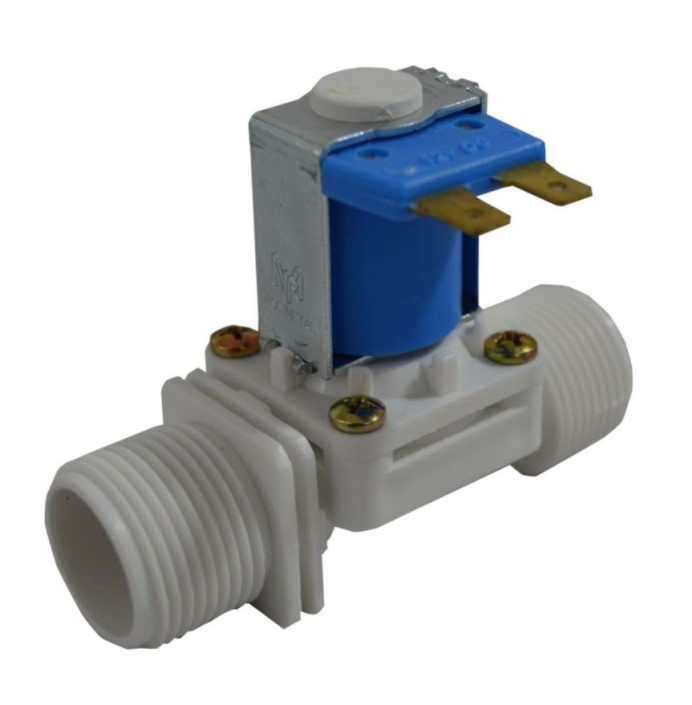
\includegraphics[width=0.3\textwidth]{figuras/solenoide.jpg}
	\fonte{Nascimetal, 2021}
	\label{fig:solenoide}
\end{figure}

\subsection{A chave de nível tipo boia}

Para questões de segurança a chave de nível \textit{RF-0H21D} foi utilizada para fomentar a redundância do sistema, caso aconteçam falhas na medição do sensor citado na seção \ref{ssec:sensor_ultra}. Essa chave indicará para o microcontrolador, por meio de contato elétrico, o momento exato para desativação da bomba d'água, evitando possíveis vazamentos no sistema acolado à caixa d'água (\textbf{TCM}). 

\begin{figure}[H]
	\centering
	\caption{Chave de nível \textit{RF-0H21D}}
	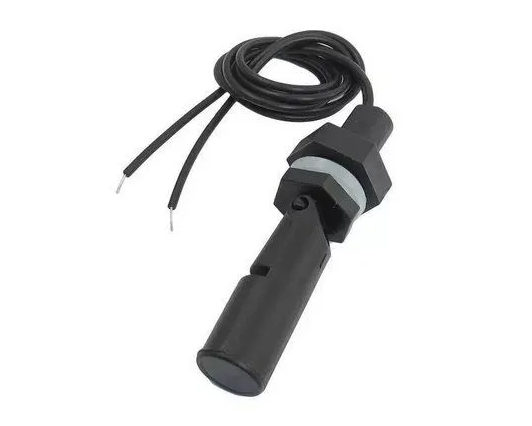
\includegraphics[width=0.5\textwidth]{figuras/chave_boia.png}
	\fonte{SMART KITS, 2020}
	\label{fig:chaveboia}
\end{figure}


\subsection{O sensor de corrente}

O sensor de corrente ACS712 selecionado é acessível e oferece precisão em soluções para detecção de corrente AC ou DC na indústria,
comercial e sistemas de comunicação. O dispositivo permite fácil implementação: aplicações típicas incluem controle de motor, detecção de carga e gerenciamento, fontes de alimentação comutadas e sobrecorrente proteção contra falhas \cite{ACS712}.


\begin{figure}[H]
	\centering
	\caption{Representação gráfica do sensor \textit{ACS712}}
	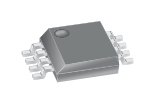
\includegraphics[width=0.3\textwidth]{figuras/ACS712.png}
	\fonte{ALEGRO, 2020}
	\label{fig:acs712}
\end{figure} 


O dispositivo consiste em um operador \textit{Hall} linear preciso, a corrente aplicada flui através do material de cobre gerando um campo magnético que é detectado pelo \textit{Hall} integrado e convertido em um proporcional de tensão. A precisão do dispositivo é otimizada por meio do fechamento proximidade do sinal magnético ao transdutor \textit{Hall}. A resistência interna do material condutor atinge uma média de \textit{1,2m}$\Omega$, proporcionando baixa potência. De acordo \textit{datasheet} do componente, pode-se observar a simples aplicação típica representada na figura abaixo.
 
\begin{figure}[H]
	\centering
	\caption{Aplicação típica do\textit{ACS712}}
	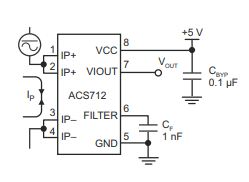
\includegraphics[width=0.4\textwidth]{figuras/ACS712_typical.png}
	\fonte{ALEGRO, 2020}
	\label{fig:acs712_typical}
\end{figure} 

\subsubsection{O sensor \textit{Hall}}

O efeito \textit{Hall} é um fenômeno que pode ser observado quando um dispositivo condutor ou semicondutor se aproxima um campo magnético perpendicular. Nessa situação uma diferença de potencial pode ser medida através dos terminais de tal dispositivo. Essa queda de tensão está relacionada com a intensidade da corrente que gerou o campo magnético \cite{ElectronicsTutorials}. A equação mostra essa relação: 

\begin{equation}
V_H = R_H\left ( \frac{I\cdot B}{t} \right)
\end{equation}

\begin{itemize}
	
	\item $V_H$ é a tensão em Volts;
	\item $R_H$ é o coeficiente do efeito \textit{Hall};
	\item  $I$ é o fluxo de corrente em Amperes;
	\item $t$ é espessura do sensor em milímetros;
	\item $B$ é a densidade do fluxo magnético em teslas; \ \\
\end{itemize}

\begin{figure}[H]
	\centering
	\caption{Comportamento da tensão de saída em relacão ao fluxo magnético de um sensor \textit{Hall}.}
	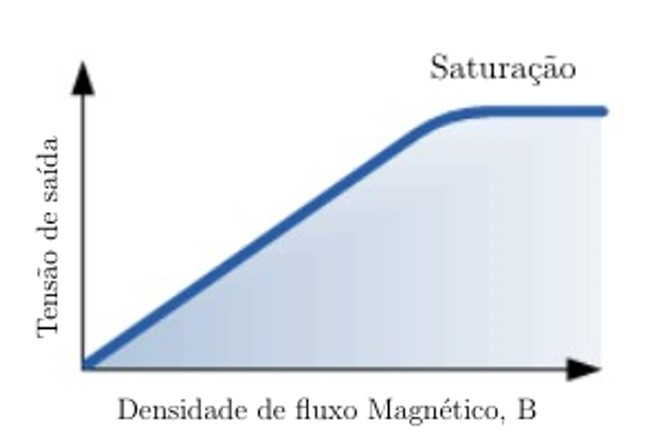
\includegraphics[width=0.4\textwidth]{figuras/grafico_hall.jpg}
	\fonte{Eletronics Tutorials, 2021}
	\label{fig:efeito_hall}
\end{figure} 

Em relação ao sensoriamento, os dispositivos \textit{Hall} podem ser digitais ou analógicos. Os sensores analógicos fornecem uma saída de tensão contínua que de acordo com a intensidade do campo magnético e em alguns casos, como o ACS712, podem apresentar uma variação de saída linear (\autoref{fig:efeito_hall}). Conforme a intensidade do campo magnético aumenta, o sinal de saída do amplificador também aumentará até que comece a saturar pelos limites impostos a ele pela fonte de alimentação do circuito integrado. Essa saída linear pode ser conectada a um pino de leitura analógica de um microcontrolador ou microprocessador.

\subsection{KiCad}

O KiCad é um \textit{Software} de código aberto para projetar circuitos eletrônicos. Essa ferramenta EDA - \textit{Electronic Design Automation} lida com captura esquemática e layout de placas de circuito impresso (PCB - \textit{Printed Circuit Board}) gerando arquivos \textit{Gerber} (padrão universal de arquivo composto de uma combinação de comandos gráficos utilizados por equipamentos tipo \textit{fotoploter} para a formação das imagens da placa de circuito impresso).

O \textit{software} roda em ambientes \textit{Windows}, \textit{Linux} e \textit{OS X} estando licenciado pela GNU GPL v3. Por meio de sua vasta biblioteca é possível construir esquemáticos de maneira prática. O KiCad também possui recursos de criação e adição de componentes, além de simulação via linguagem SPICE (ainda em beta) \cite{Kicad}. 

\begin{figure}[H]
	\centering
	\caption{Exemplo de\textit{PCB Design} utilizando \textit{Kicad}}
	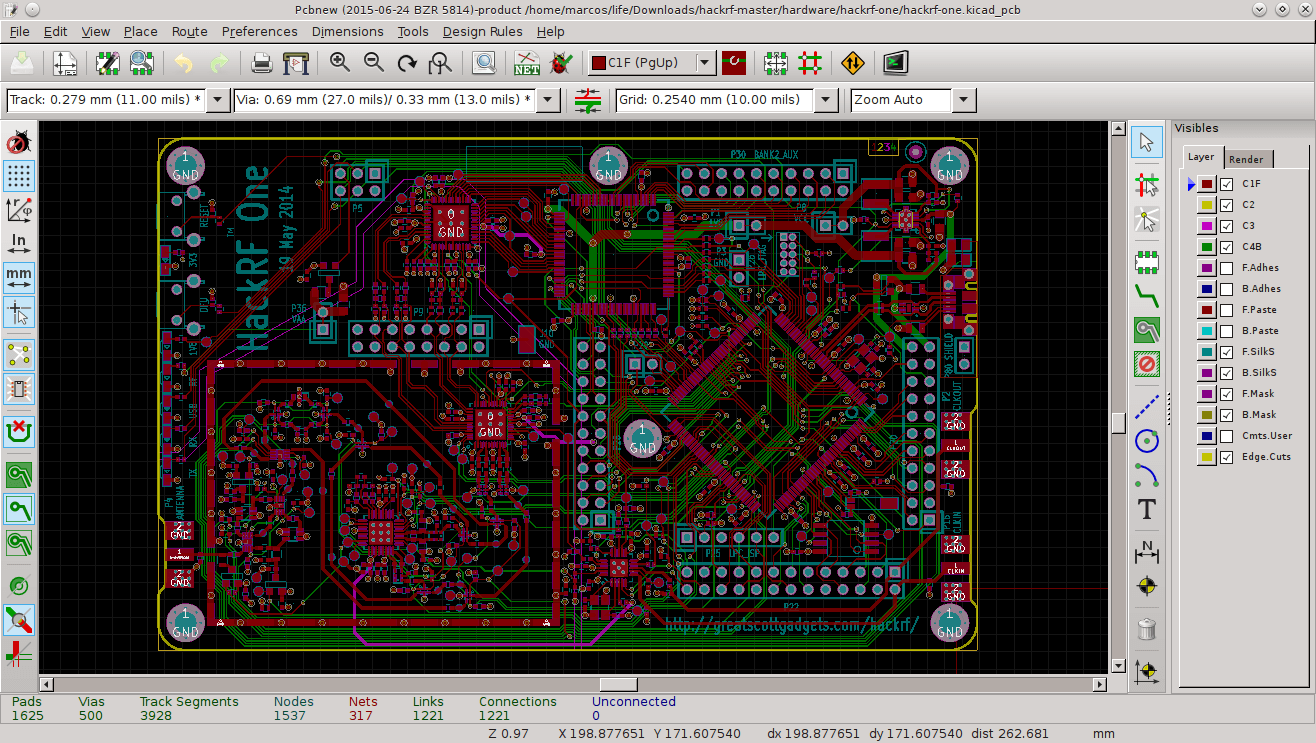
\includegraphics[width=0.6\textwidth]{figuras/kicad_pcbnew.png}
	\fonte{kicad.org, 2021}
	\label{fig:kicad_pcbnew}
\end{figure} 


%\subsection{Autocad Inventor}

\section{Elementos de \textit{Firmware}}

\subsection{O Ambiente de Desenvolvimento \textit{PlatformIO}}


O \textit{PlatformIO} é uma ferramenta profissional de plataforma cruzada, ou seja, disponível em diversas plataformas de desenvolvimento, e de estrutura múltipla voltada para desenvolvedores de \textit{software} embarcado.

A ferramenta (\autoref{fig:platformio}) fornece um ambiente de desenvolvimento integrado moderno, oferecendo suporte a diversos \textit{kits} de desenvolvimento de \textit{software} (\textit{SDKs}) ou \textit{frameworks} e inclui depuração sofisticada (\textit{Debug Mode}), testes de unidade (\textit{Unit Test}), análise automatizada de código (\textit{Static Code Analysis}) e gerenciamento remoto (\textit{Remote Development}). É arquitetado para maximizar a flexibilidade e escolha dos desenvolvedores, que podem usar editores gráficos e/ou de linha de comando (\textit{PlatformIO Core}(\textit{CLI})).

Com esta interface, será possível a programação do microcontrolador \textit{ESP8266} através da linguagem \textit{C++} em conjunto com todas as bibliotecas disponibilizadas pela plataforma Arduino. Todas as funcionalidades, como rotinas de conexão \textit{HTTP} e/ou \textit{MQTT} através do \textit{Wi-Fi}, Interrupção, \textit{Timers} e Modos de Energia são completamente acessíveis. 

\begin{figure}[H]
	\centering
	\caption{Extensão do \textit{PlatformIO} rodando no \textit{Visual Studio Code}}
	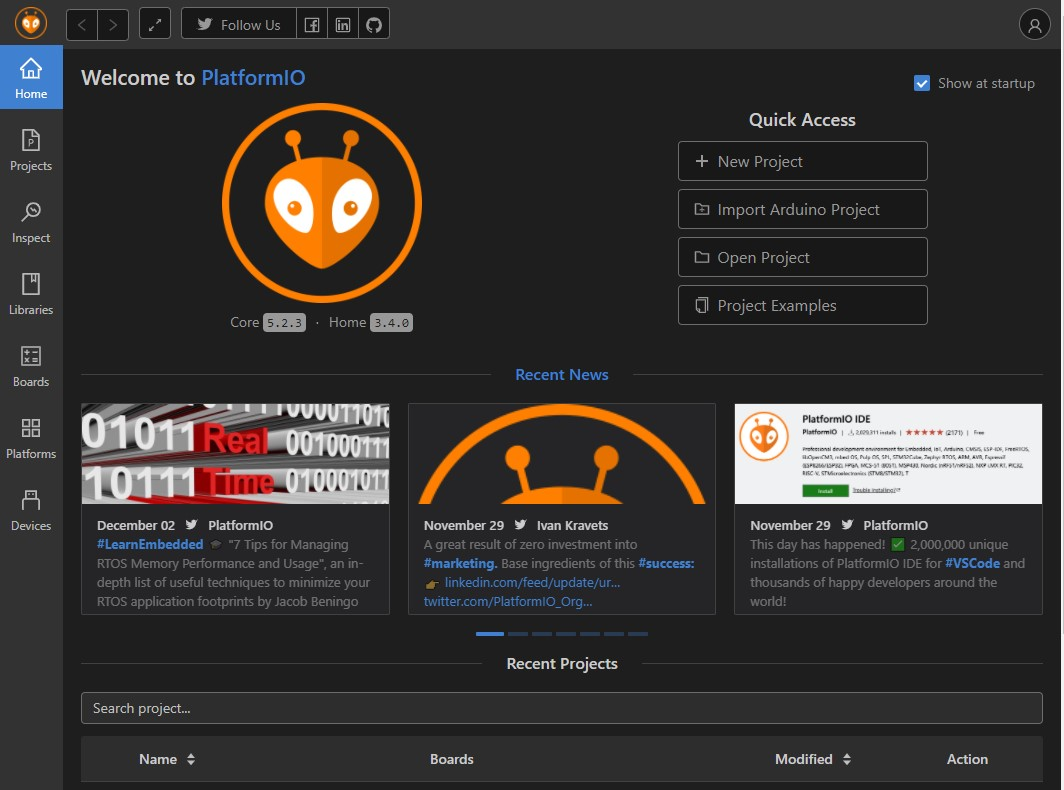
\includegraphics[width=0.7\textwidth]{figuras/platformio.jpg}
	\fonte{Própria, 2021}
	\label{fig:platformio}
	
\end{figure}


\subsection{\textit{Linux} embarcado e a distribuição \textit{DietPi}}

\textit{Linux} é um sistema operacional de código aberto amplamente utilizado em vários sistemas, possuindo compatibilidade com diversos tipos de microprocessadores, sejam eles de arquitetura \textit{Reduced Instruction Set Computer} - RISC ou \textit{Complex Instruction Set Computer} - CISC. Em todos os casos executa rotinas por baixo de todos os outros \textit{softwares}, gerenciando todas as ações em conjunto com \textit{hardware}.

O termo “\textit{Linux}” tecnicamente se refere apenas ao \textit{kernel} do \textit{Linux}. A maioria das pessoas se refere a todo o sistema operacional como \textit{"Linux"} porque, para a maioria dos usuários, um sistema operacional inclui um pacote de programas, ferramentas e serviços (como desktop, relógio, menu de aplicativo e assim por diante). Algumas pessoas, particularmente membros da \textit{Free Software Foundation} , referem-se a esta coleção como \textit{GNU / Linux} , porque muitas ferramentas vitais incluídas são componentes \textit{GNU}. No entanto, nem todas as distribuições do \textit{Linux} usam componentes \textit{GNU} como parte do sistema operacional: o \textit{Android} , por exemplo, usa um \textit{kernel Linux}, mas depende muito pouco das ferramentas \textit{GNU} \cite{opensource}.

O mesmo \textit{Linux} que roda em um supercomputador pode rodar também em uma simples placa eletrônica. O que torna isso possível é que o \textit{Linux} suporta uma grande variedade de arquiteturas e processadores \cite{SoftwareLivre}. Baseado na distribuição em Debian, conhecida por sua alta confiabilidade, a distribuição \textbf{DietPi}, utilizada neste trabalho, é extremamente leve, sendo altamente otimizada para o uso mínimo de recursos de CPU e RAM, garantindo que a \textit{Central Process Unit} - CPU sempre opere em seu potencial máximo. Essa distribuição é suportada por diversos microprocessadores, incluindo o Broadcom BCM2835, presente na Raspberry PI Zero W.

\begin{figure}[H]
	\centering
	\caption{Catálogo com algumas de placas que suportam a distribuição DietPi.}
	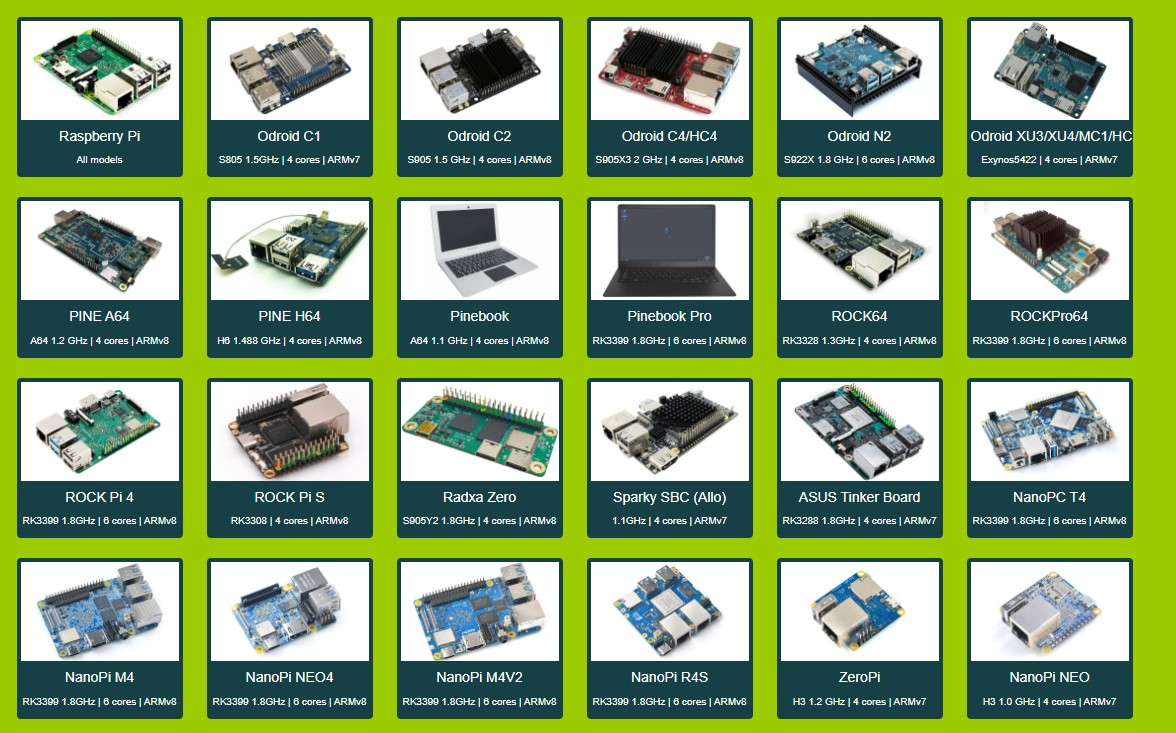
\includegraphics[width=0.7\textwidth]{figuras/dietpi.jpg}
	\fonte{dietpi.com, 2021}
	\label{fig:dietpi}
\end{figure} 


\section{Elementos de \textit{Software}}

\subsection{Figma}

Figma é um editor gráfico de prototipagem para projetos de \textit{design} baseado principalmente no navegador web, com ferramentas \textit{offline} adicionais para aplicações \textit{desktop}, \textit{GNU/Linux}, \textit{macOS} e \textit{Windows}. Possui também a ferramenta \textit{Figma Mirror}: um sistema de prototipagem que espelha o que está sendo feito no computador para o \textit{smartphone} \textit{Android} e/ou \textit{iOS,} permitindo a simulação do desenho criado, como um aplicativo ou página da web. Por meio desse \textit{software} é possível criar e manipular animações e transições de telas, focando no desenvolvimento de \textit{User Interface Experience} - UI/UX \cite{Figma}.

\begin{figure}[H]
	\centering
	\caption{Exemplo de um projeto desenvolvido no Figma.}
	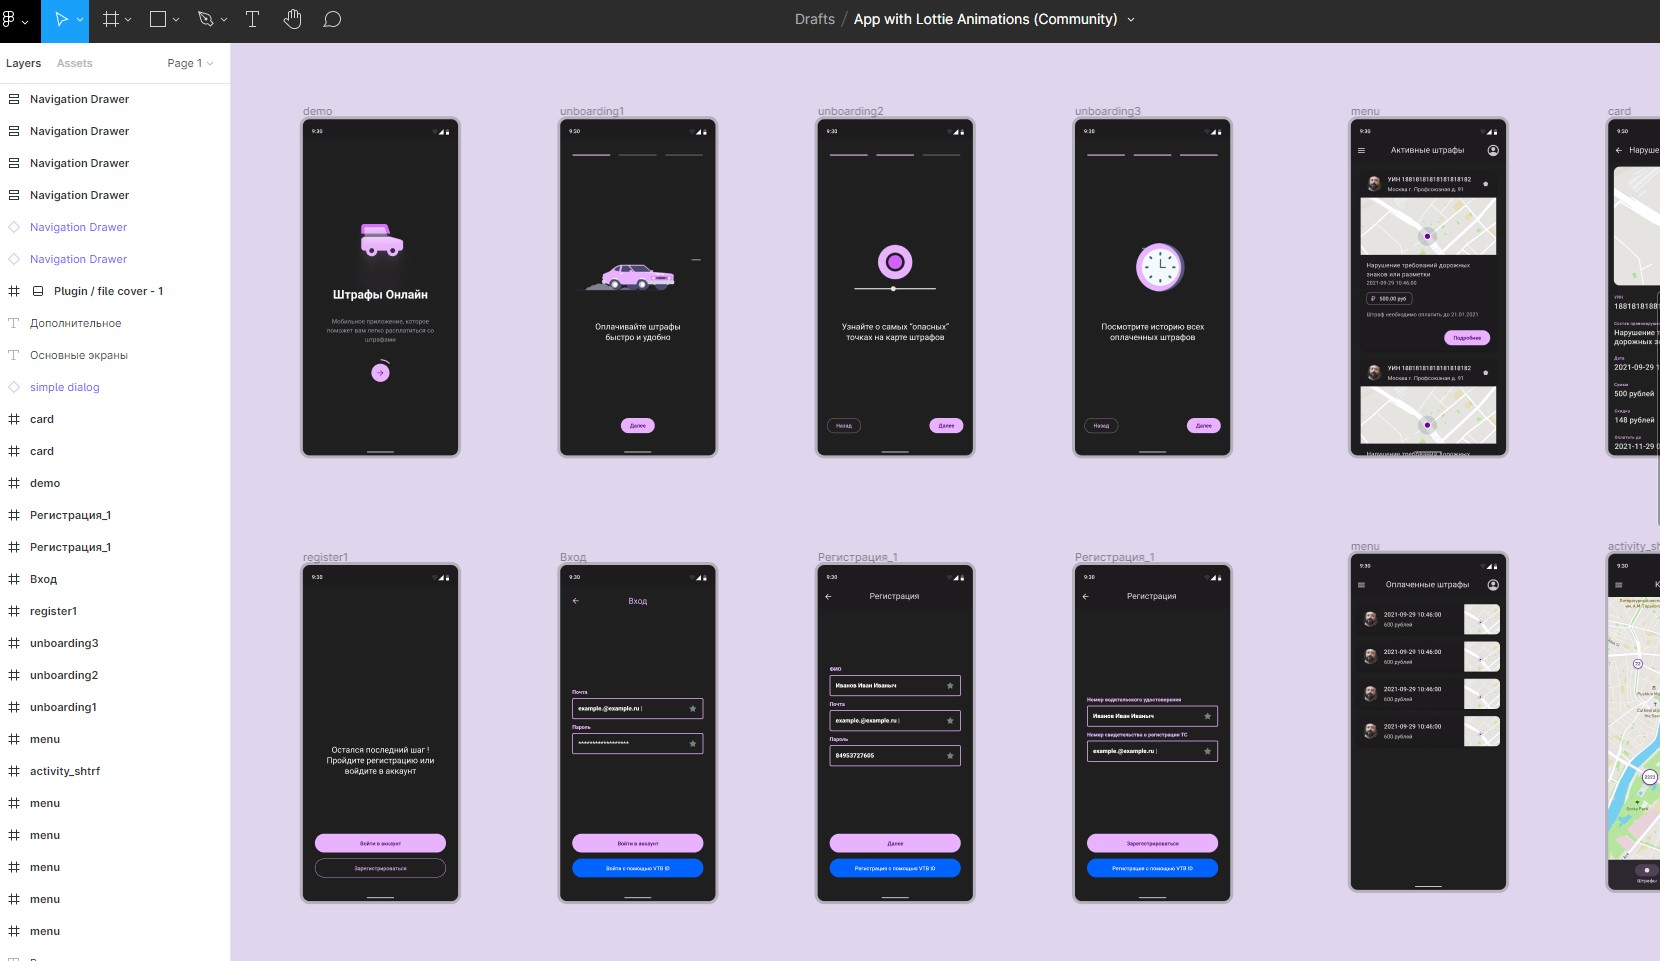
\includegraphics[width=0.7\textwidth]{figuras/figma_exemplo.jpg}
	\fonte{figma.com, 2021}
	\label{fig:figma_exemplo}
\end{figure} 



\subsection{\textit{Node.js}}

O \textit{Node.js} é um ambiente de execução (\textit{runtime}) \textit{Javascript} possibilitando criar aplicações sem depender de um \textit{browser} para a execução. Por meio desta tecnologia, se torna possível empregar o \textit{Javascript} para executar comandos em terminal assim como utilizá-lo para programar qualquer tipo de aplicação \textit{backend} com auxílio de inúmeras bibliotecas desenvolvidas. As bibliotecas do \textit{Node.js} podem ser acessadas e instaladas por seu gerenciador de pacote oficial, o \textit{Node Package Manager} - \textbf{NPM} \cite{NodeJs}.


\subsection{\textit{Electron}}

O \textit{Electron} é um \textit{framework} multiplataforma (Windows, Linux e MacOS) para criação de interfaces possibilitando o usuário acessar serviços do sistema operacional tanto via linha de comando - \textit{CLI} e interface gráfica - \textit{GUI} \cite{Electron}.

\begin{figure}[H]
	\centering
	\caption{Aplicações que utilizam \textit{Electron}}
	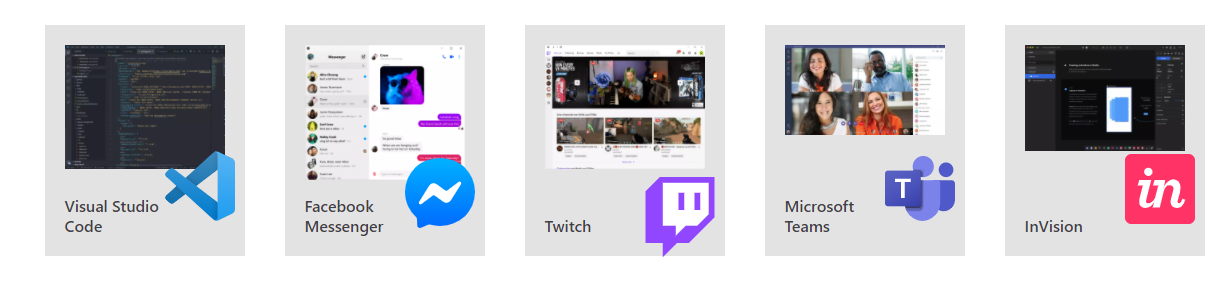
\includegraphics[width=1.0\textwidth]{figuras/electron_apps.png}
	\fonte{Adaptado (electronjs.org, 2020)}
	\label{fig:electron_apps}
\end{figure} 

Por meio dele podemos desenvolver aplicações \textit{desktop} utilizando \textit{HTML}, \textit{CSS}, \textit{Javascript} em conjunto com todas as ferramentas aplicadas a um desenvolvimento \textit{frontend web}. Incorporando o \textit{Chromium}, navegador de código aberto \cite{Chromium}, e \textit{Node.js} no seu binário, toda a base de código fica por conta do \textit{JavaScript} eliminando a experiência de desenvolvimento nativo.

Uma aplicação \textit{Electron} tem como base os seguintes arquivos:

\begin{itemize}
	\item \textbf{\textit{package.json}}: Aponta para o arquivo principal do aplicativo e lista seus detalhes e dependências;
	\item \textbf{\textit{main.js}}: Inicia a aplicação e cria a janela de visualização possibilitando diversas configurações; 
	\item \textbf{\textit{index.html}}: O ponto de partida para a renderização.
\end{itemize}



\subsection{\textit{React}}

O \textit{React} é uma biblioteca \textit{JavaScript}, desenvolvida pela equipe do \textit{Facebook}, que possui ferramentas que facilitam a construção de Interfaces na \textit{Web}. Ele transforma um ambiente complexo, cheio de \textit{Edge Cases} (casos onde você precisa tratar eventos e como os dados são manipulados) em algo muito mais simplificado \cite{React}.

Trabalhando no contexto declarativo, essa biblioteca permite criar telas para cada estado da aplicação, atualizando e renderizando apenas os itens necessários de forma eficiente. Os itens podem ser componentes (arquivos \textit{JSX}) encapsulados que gerenciam seu próprio estado.

\textit{JSX} é uma forma de criar elementos para serem utilizadas como \textit{templates} de aplicações \textit{React}. São bem similares ao código \textit{HTML}, porém, não é interpretado pelo navegador. Por este motivo, deve-se utilizar um transpilador \footnote{\textbf{transpilador}: subconjunto de compiladores os quais identificam um arquivo de código-fonte e o convertem em outro arquivo de código-fonte, sendo de outra linguagem ou em uma versão diferente da mesma linguagem.} para essa conversão. Atualmente, o mais conhecido deles é o \textit{Babel}.

\begin{figure}[H]
	\centering
	\caption{Exemplo de componente \textit{React}}
	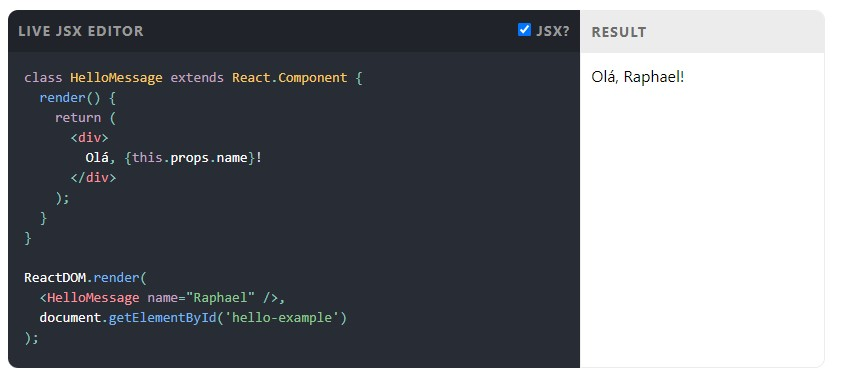
\includegraphics[width=0.8\textwidth]{figuras/exemplo_react.jpg}
	\fonte{Adaptado (reactjs.org, 2021)}
	\label{fig:react_code}
\end{figure} 


\subsection{\textit{React Native}}

Baseado no \textit{React}, para desenvolvimento \textit{WEB}, o \textit{React Native} é um \textit{framework} de codigo aberto desenvolvido pela equipe do \textit{Facebook} que suporta a criação de aplicativos \textit{mobile} multiplataforma (Android e iOS), sem que haja a preocupação de lidar com as linguagens padrões como \textit{Java} ou \textit{Swift}, usando apenas \textit{Javascript}. Como ponto positivo, ao contrário de outros \textit{frameworks} com o mesmo propósito, todo código desenvolvido com \textit{React Native} será convertido para a linguagem nativa do sistema operacional, o que torna a aplicação mais rápida.

\begin{figure}[H]
	\centering
	\caption{Exemplos de \textit{Templates} produzidos com \textit{React Native}}
	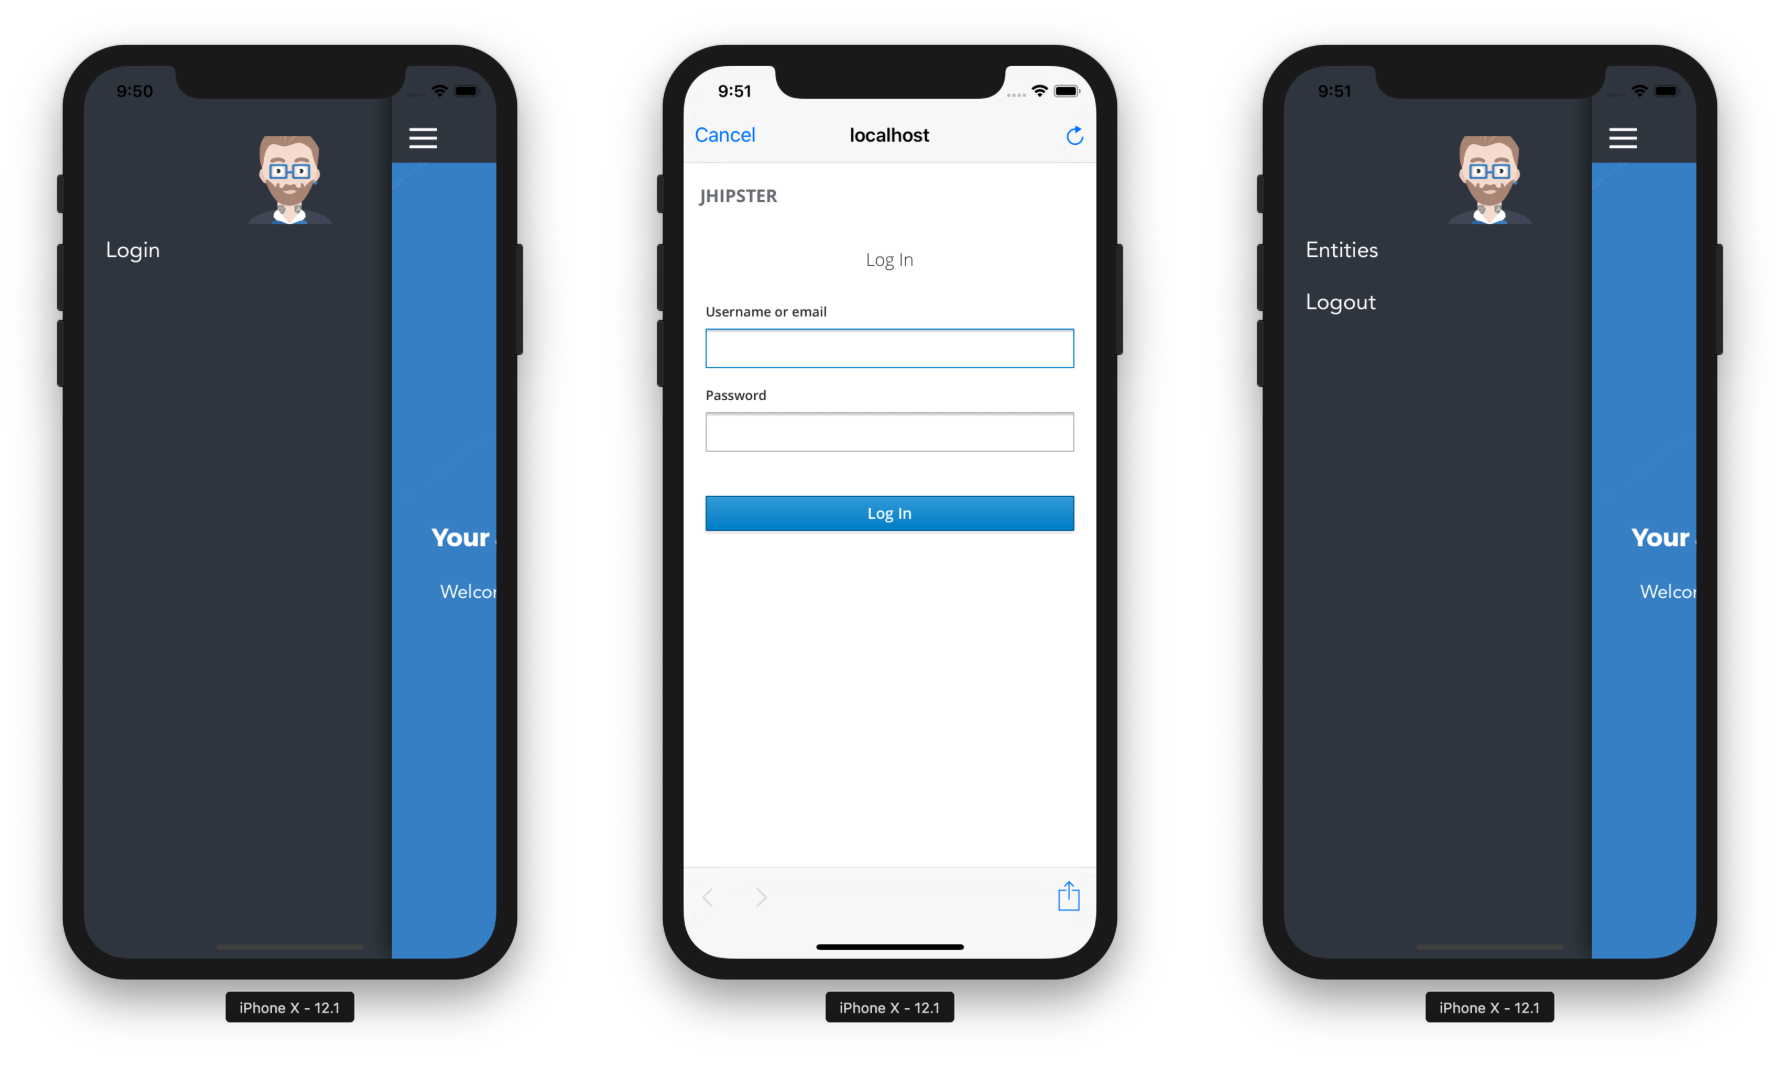
\includegraphics[width=0.7\textwidth]{figuras/react_native_elements.png}
	\fonte{Adaptado (developer.oka, 2021)}
	\label{fig:react-native}
\end{figure} 

